\documentclass[12pt, titlepage]{article}

\usepackage{graphicx}
\usepackage{wrapfig}
\usepackage{hyperref}
\usepackage{siunitx}
\usepackage{amsmath}
\usepackage{enumerate}

\title{Flippin' Flingers Trebuchet Final Report}
\author{Omar Ebrahim 110076575\\Saif Kaoud 110076323\\[10pt] Dr. John Magliaro\\
University of Windsor}

\begin{document}
    \maketitle
    \section{Abstract}
    This final report provides an overview of the finalization of the project focused on the sketching, designing, and modeling of a trebuchet.\\[10pt]
    The report outlines the key milestones achieved since the inception of the project, 
    including build process, changes from the initial design, detailed component specifications, analytical-numerical-physical test results, and dicussion on test results.\\[10pt]
    The report utilizes CAD, first principles, numerical simulations, and physical tests to achieve this goal.
    \newpage
    \tableofcontents
    \listoffigures
    \newpage
    \section{Introduction}
    This report's mission statement is to summarize the team's final results with:
    \begin{itemize}
        \item Detailed CAD drawings.
        \item Analytical Calculations.
        \item Numerical modeling.
        \item Real-life data.
    \end{itemize}
    The problem outline is to design and analyze the trebuchet to maximize
    projectile distance and accuracy.\\[10pt]
    The trebuchet is designed for maximum distance through general
    plane motion.\footnote{Hibbeler, 2015}It is also designed for maximum 
    accuracy through string measure.\footnote{Rhoten, 2021}\\[10pt]
    To maximize distance, the velocity of the projectile is considered, as
    distance and velocity are proportional. Increasing the counterweight 
    fall distance can boost the projectile's velocity.\footnote{Siano, 2001}
    Increasing the counterweight-to-launch distance increases the velocity 
    of the projectile.\footnote{Denny, 2005}\\[10pt]
    Lastly, adjusting the trebuchet firing angle to 
    45 degrees achieves the maximum projectile distance.\footnote{Connel, 2001}
    \newpage
    \section{Methodology}
    The team uses CATIA, a CAD software, to design components and present
    them in detailed technical drawings.\\[10pt] 
    Next, the team applies the principles of Kinematics and Kinetics to analyze the motion of the trebuchet. 
    Through this analysis, they are able to make accurate estimations regarding the distance the projectiles will travel.\\[10pt]
    The team also utilizes Working Model 2D, a CAE software, to numerically simulate the trebuchet's motion and provide numerical data for analyzing the impact of various factors on its performance.\\[10pt]
    Finally, the team conducts real-life tests of the trebuchet to compare and contrast the actual results with their analytical and numerical predictions. They carefully analyze the variations between the expected and observed outcomes, discussing the factors that contribute to these differences.    
    \newpage
    \section{Design}
    Figure \ref{CAD} showcases the CAD model of the Floating Arm Trebuchet. The design features a robust physical body. The counterweight is attachable to the middle axle, and the arm holds the sling and guide chute at the end. To enhance portability, wheels are attachable to the corners of the base, facilitating easy transportation of the trebuchet.\\
    \begin{figure}[t]                                  
    \centering
    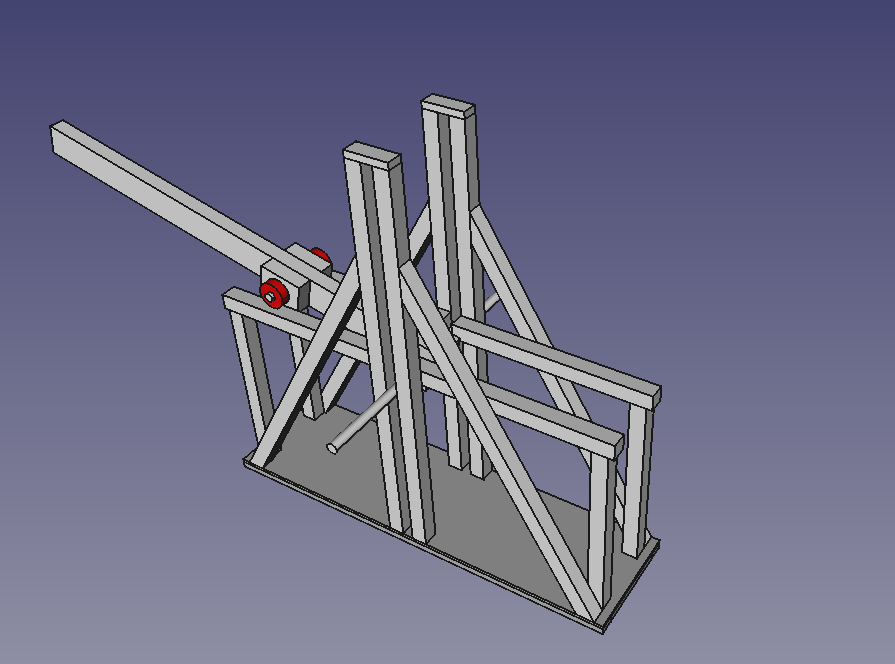
\includegraphics[width=0.8\textwidth]{figures/CAD.png}
    \caption{Floating Arm Trebuchet in CAD\label{CAD}}
    \end{figure}
    \newpage
    \subsection{Technical Drawings}
    \begin{figure}[b]
    \begin{minipage}[t]{0.45\textwidth}
        \begin{flushleft}
            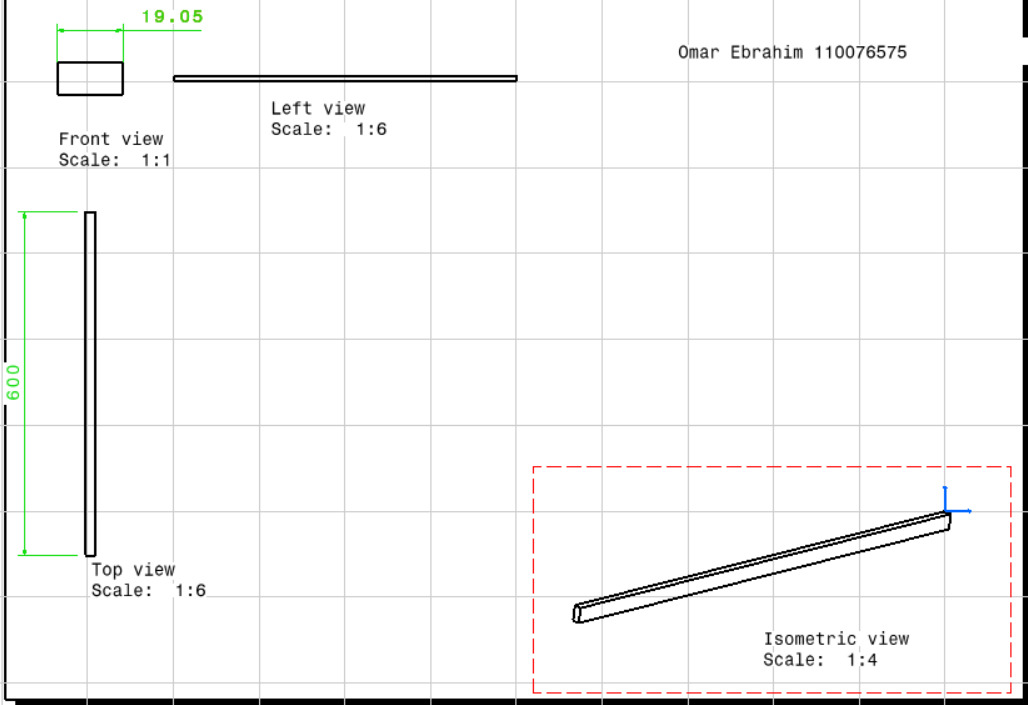
\includegraphics[width=\textwidth]{figures/Drawing1.jpeg}
        \end{flushleft}
        \caption{60 cm rod\label{60rod}}
    \end{minipage}
    \hfill
    \begin{minipage}[t]{0.45\textwidth}
        \begin{flushright}
            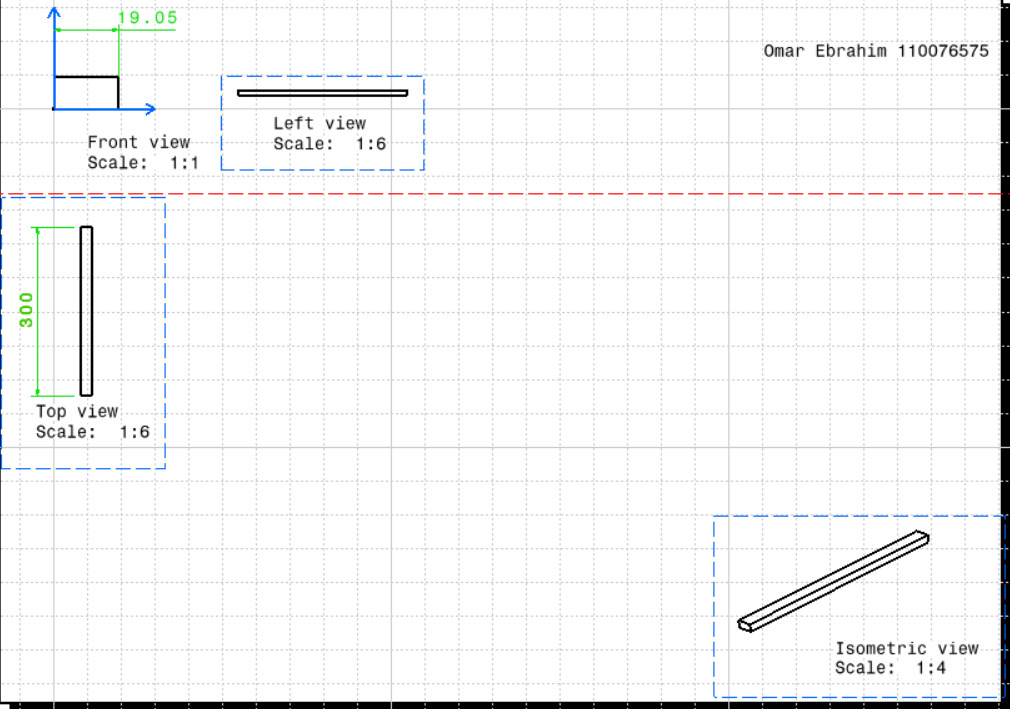
\includegraphics[width=\textwidth]{figures/Drawing2.jpeg}
        \end{flushright}
        \caption{30 cm rod\label{30rod}}
    \end{minipage}
    \end{figure}
    The trebuchet's structural body is designed using two main components: 60 cm and 30 cm wooden
    rods. The 60 cm rods are used for the base length, arm, ramp, and uprights. While 
    the 30 cm rods are used for the base width and frame. \\[10pt]
    The design is very simple yet effective. The team used CATIA to design 
    and create drafts for these components. Technical drawings for these 
    components are shown in Figures \ref{60rod} and \ref{30rod}.\\[10pt]
    The technical drawings showcase the front, top, left, and isometric views of the components.
    The wooden rods are the same dimensions except their length, so the width and height 
    of the rods are 3/4" 3/8" or 1.905 cm 0.9525 cm respectively.
    \newpage
    \section{Results}
    \subsection{Analytical Calculations}
    \begin{figure}[b]                                  
    \centering
    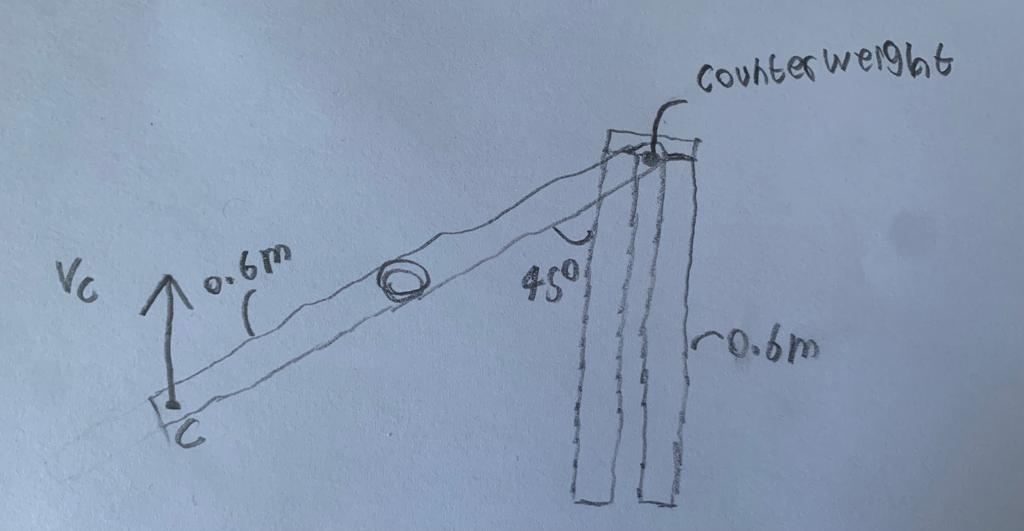
\includegraphics[width=0.45\textwidth]{figures/d1.jpeg}
    \caption{Diagram\label{d1}}
    \end{figure}
    Before the team can begin to analyze the motion of the trebuchet, they must
    first take some measurements. The team measures the length of the arm to be 
    approximately $0.6$ m. The team uses two 355mL drink cans.
    Therefore, the mass of the counterweight is $\frac{2*355}{1000} \approx 0.7$ kg.
    The mass of the arm with the supporting wheels is $0.3$ kg.
    Hence, the combined mass of the counterweight with the arm is 
    $0.7 + 0.3 = 1$ kg. The team measured the radius
    and height of the cans which were $0.066$ m and $0.12$ m respectively. See Figure \ref{d1}.\\[20pt]
    Given: $m_{a} = 0.3$ kg, $m_{w} = 0.7$ kg, $m = 1$ kg, $l = h = 0.6$ m, $\theta = 45^\circ$
    $r = 0.066$ m and $h_c = 0.12$ m\\
    RTF: Range of projectile, $s$\\
    Assumptions: Rigid bodies, no energy loss, starts from rest.\\[10pt]
    To solve this problem, the team uses the General Work-Energy Equation:
    $$T_1 + \Sigma U_{1-2} = T_2$$
    Since, the trebuchet starts from rest, $T_1 = 0$. Now, to find $\Sigma U_{1-2}$,
    $$\Sigma U_{1-2} = mgh = (1)(9.8)(0.6) = 5.88 \approx 5.9 \mathrm{J}$$
    To find $T_2$, the team needs to find the equivalent mass moment of inertia $I_e$,
    $$I_e = I_a + I_w$$
    \newpage
    \noindent The team assumes the arm to be a rod, and the counterweight to be a cylinder. Therefore,
    \begin{align*}
        I_e &= \frac{1}{12}m_al^2 + \frac{1}{12}m_w(3r^2 + h_c^2) \\
        &= \frac{1}{12}(0.3)(0.6)^2 + \frac{1}{12}(0.7)\left(3(0.066)^2 + (0.12)^2\right) = 0.0106 \, \mathrm{kg} \cdot \mathrm{m}^2
    \end{align*}
    To find $T_2$ we need to relate $\omega$ with v, the team uses the kinematic equation for rotational motion,
    $$v = \omega l;\; \omega = \frac{v}{l}$$
    Substituting this into the kinetic energy equation,
    \begin{align*}
        T_2 &= \frac{1}{2}mv^2 + \frac{1}{2}I_e\left(\frac{v}{l}\right)^2 \\
        &= \frac{1}{2}(1)v^2 + \frac{1}{2}(0.0106)\left(\frac{v}{0.6}\right)^2 \\
        &= 0.5v^2 + 0.0147v^2 = 0.5147v^2
    \end{align*}
    Now, substituting $\Sigma U_{1-2}$ and $T_2$ into the General Work-Energy Equation,
    $$5.9 = 0.5147v^2$$
    $$v = v_e = 3.38 \, \mathrm{m/s};\; \omega = \frac{3.38}{0.6} = 5.63 \, \mathrm{rad/s}$$
    Now, to find the velocity of point C, the team uses the kinematic equation for rotational motion assuming the distance from the equivalent center to point C is $0.5$ m,
    $$v_c = v_e + \omega l_{c/e} = 3.38 + (5.63)(0.5) = 6.2 \, \mathrm{m/s}$$
    Now, to find the range of the projectile, the team uses the parabolic motion equation assuming that the time right before the ball lands is 4 seconds,
    $$v_c = \frac{ds}{dt};\; \displaystyle\int_{0}^{s}ds = \displaystyle\int_{0}^{4}6.2dt$$
    \[ \boxed{s = 24.8 \, \mathrm{m}} \]
    From this analysis, the team predicts that the trebuchet will launch the projectile 24.8 meters.
    \newpage
    \subsection{Numerical Model}
    The Floating Arm Trebuchet implemented in Working Model 2D can be found 
    in Figure \ref{model}. Additionally, a tracing of the trebuchet's motion 
    can be found in Figure \ref{motion}. Tracing is a feature in Working 
    Model 2D that shows each frame of the motion of an object.\\[5pt]
    The simulation creates a P-V-A graph as shown in Figure \ref{graphs}.
    The parameters used in the simulation are as follows: $m_{w} = 0.7$ kg, $l_{arm} = h = 0.6$ m,
    $\theta = 45^\circ$, and $r_{circle} = 0.066$ m. As shown in the graph, the ball's 
    velocity is initially zero, decreases then increases to its maximum velocity at time $t = 1.5$ s.
    The ball's position increases as it is launched until it reaches the ground after 4 seconds. By looking at the x direction graph at t = 4 s, 
    the team predicts that the range of the projectile is approximately 24 meters.

    \begin{figure}[t]                                  
    \centering
    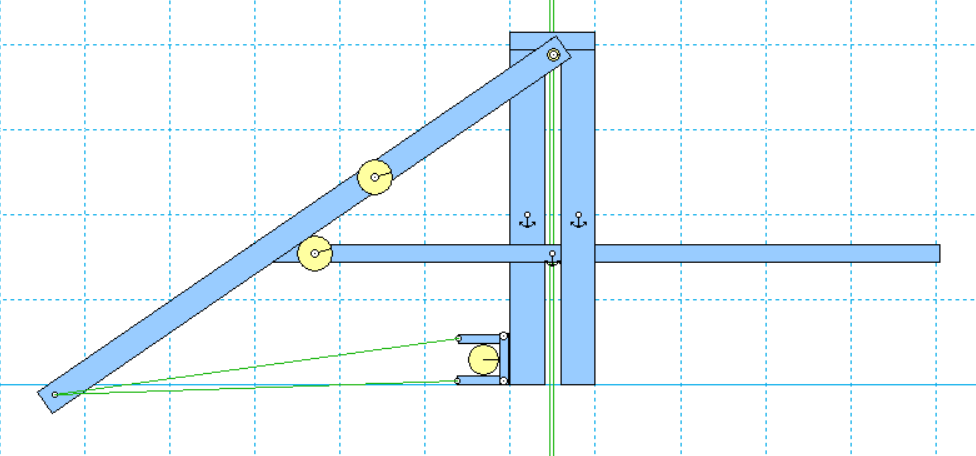
\includegraphics[width=0.7\textwidth]{figures/Model.png}
    \caption{Floating Arm Trebuchet model in Working Model 2D\label{model}}
    \end{figure}

\begin{figure}[b]
    \begin{minipage}[t]{0.69\textwidth}
        \vspace{12pt}
        \begin{flushleft}
            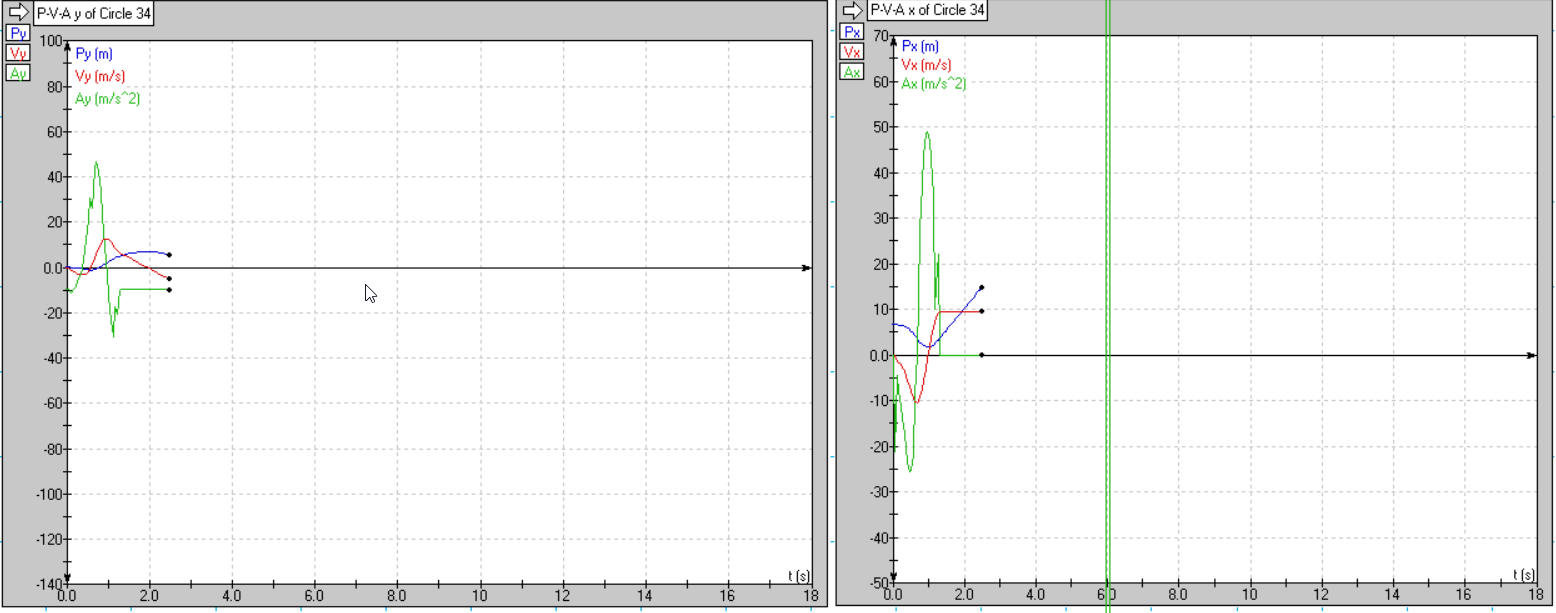
\includegraphics[width=\textwidth]{figures/Graphs.png}
        \end{flushleft}
        \caption{P-V-A graph of ball\label{graphs}}
    \end{minipage}
    \hfill
    \begin{minipage}[t]{0.3\textwidth}
        \vspace{50pt}
        \begin{flushright}
            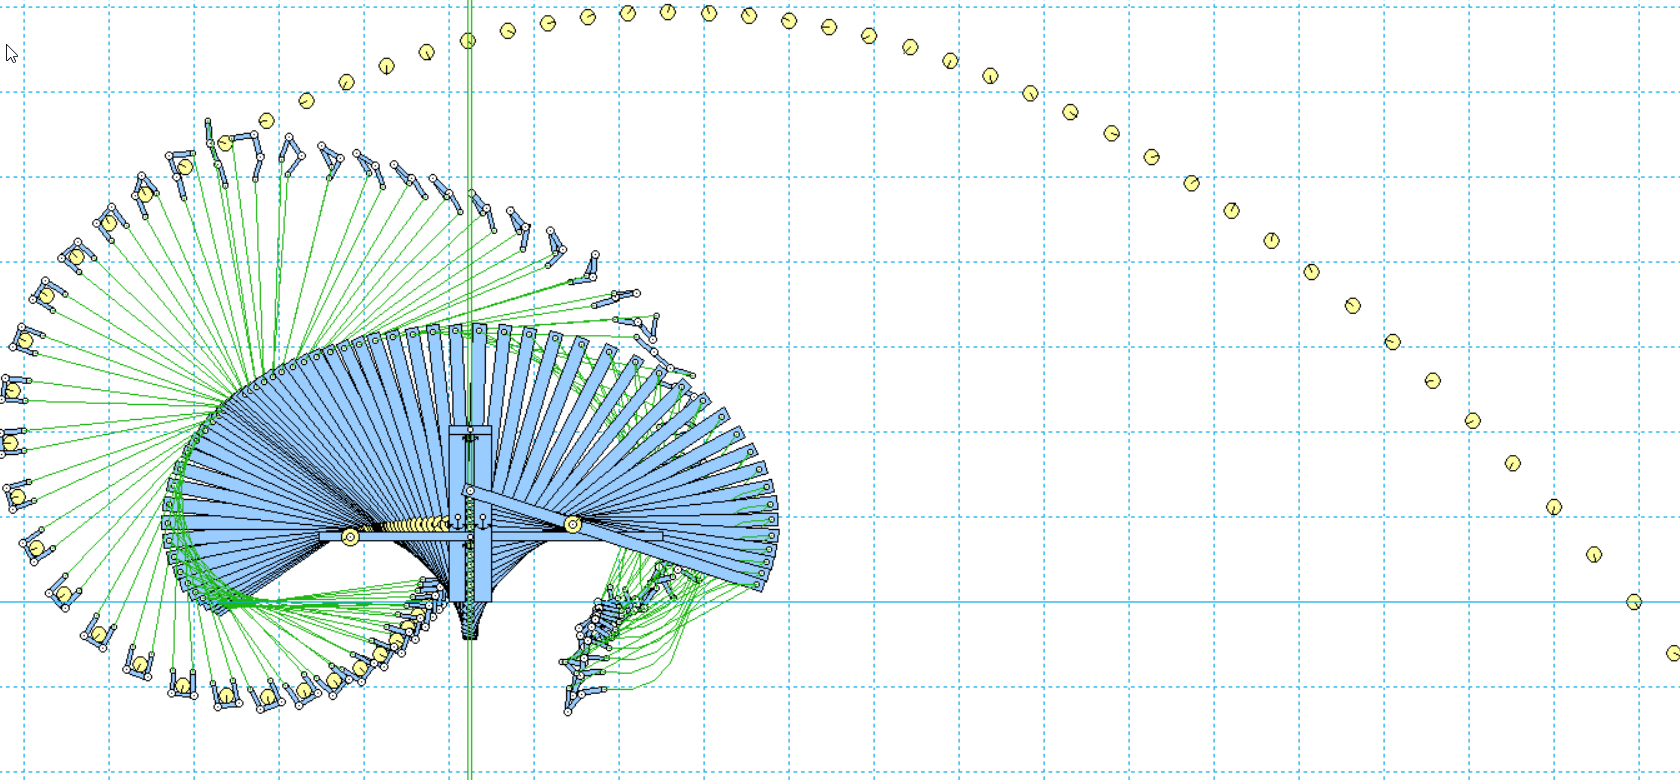
\includegraphics[width=\textwidth]{figures/Motion.png}
        \end{flushright}
        \caption{Motion of Trebuchet\label{motion}}
    \end{minipage}
    \end{figure}
    \newpage
    \subsection{Real-life Data}
    \begin{figure}[b]                                  
    \centering
    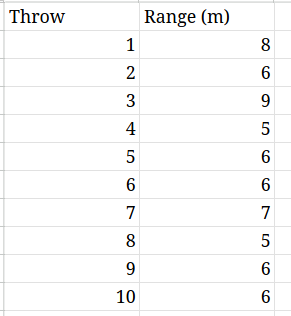
\includegraphics[width=0.32\textwidth]{figures/table.png}
    \caption{Data of 10 throws\label{table}}
    \end{figure}
    The team conducted a real-life experiment to test the range of the
    trebuchet. The results can be found in Figure \ref{table}.\\[10pt]
    The team uses the mean of the data to find the average range of the
    that the projectile traveled. The mean is calculated as follows:
    \begin{align*}
        \bar{x} = \frac{1}{n}\sum_{i=1}^{n}x_i = \frac{2*5 + 5*6 + 7 + 8 + 9}{10} = 6.4  \, \mathrm{m}
    \end{align*}
    Hence, to find the efficiency of the trebuchet, the team uses the following equation:
    \begin{align*}
        \eta = \frac{\mathrm{Actual\;Range}}{\mathrm{Predicted\;Range}} = \frac{6.4}{24.8} = 0.258
    \end{align*}
    Therefore, the team concludes that the trebuchet is 25.8\% efficient.
    \newpage
    \section{Comparison of Results}
    To compare the results of the analytical calculations, numerical model, and the real-life data the team uses this equation:
    \begin{align*}
        \mathrm{Percent\;Error} = \frac{\mathrm{Predicted\;Range} - \mathrm{Actual\;Range}}{\mathrm{Predicted\;Range}} * 100\%
    \end{align*}
    \subsection{Analytical/Numerical}
    The team starts by comparing the analytical calculations and the numerical model. The team uses the following equation to find the percent error:
    \begin{align*}
        \mathrm{Percent\;Error} = \frac{24.8 - 24}{24.8} * 100\% = 3.226\%
    \end{align*}
    \subsection{Analytical/Real-life}
    Now to find the percent error between the analytical calculations and the real-life data, the team uses the following equation:
    \begin{align*}
        \mathrm{Percent\;Error} = \frac{24.8 - 6.4}{24.8} * 100\% = 74.2\%
    \end{align*}
    \subsection{Numerical/Real-life}
    Lastly to find the percent error between the numerical model and the real-life data, the team uses the following equation:
    \begin{align*}
        \mathrm{Percent\;Error} = \frac{24 - 6.4}{24} * 100\% = 73.3\%
    \end{align*}
    \newpage
    \section{Discussion}
    From the Comparison of Results section, the team concludes that the 
    analytical calculations and numerical model are very similar because
    they have a percent error of 3.226\%. This is because both the 
    analytical calculations and numerical model use the same principles.
    \subsection{Limitations}
    The real-life data is very different from both the analytical calculations
    and numerical model. This is because the real-life data is affected by
    many factors such as wind, friction, and the release angle. These 
    factors are not taken into account in the analytical calculations and
    numerical model.\\[10pt]
    These results don't discredit the analytical calculations and numerical
    model because these calculations and models are based on the ideal
    conditions.\\[10pt]
    The analytical calculations and numerical model help the team to find 
    the best case scenario for the trebuchet. The team can use this 
    to make meaningful predictions about how the trebuchet will perform.
    \subsection{Improvements}
    The team can improve the design of the trebuchet by approaching the
    ideal conditions. The team can do this by reducing the friction between
    the projectile and the sling as well as increase the time of release.\\[10pt]
    To deal with friction, the team can use a lubricant on key parts that 
    are affected by friction. To increase the time of release, the team can
    use a longer sling and tweak the trebuchet to release the projectile 
    at 45 degrees.
    \newpage
    \section{Conclusions}
    The main objectives of this milestone were to provide updated detailed
    technical drawings, calculate the range of the projectile using 
    analytical calculations and numerical models, compare the results,
    and discuss the limitations and improvements of the design.\\[10pt]
    The key findings are summarized as follows:
    \begin{enumerate}
        \item To maximize distance, the velocity of the projectile should be
        considered because the range of the projectile is proportional to
        the velocity.
        \item The analytical calculations and numerical model predictions are 
        very similar. The analytical calculations predict that the projectile
        will travel 24.8 meters while the numerical model predicts that the
        projectile will travel 24 meters.
        \item The average range of the projectile in the real-life experiment
        is 6.4 meters. This is very different from the analytical calculations
        and numerical model. This is because the real-life experiment is
        affected by many factors such as wind, friction, and the release angle.
        \item To improve the design of the trebuchet, the trebuchet
        should be tweaked to approach the ideal conditions. This can be done
        by reducing friction and increasing the time of release.
    \end{enumerate}
    \newpage
    \section{References}
        \hspace{15pt}Denny, M. (2005). Siege engine dynamics. European journal of physics, 26(4), 561.

        Hibbeler, R. C. (2015). 16.5. In Engineering mechanics: Dynamics (pp. 346–348). essay, Pearson.
        
        James O'Connell; Dynamics of a medieval missile launcher: the trebuchet. The Physics Teacher 1 November 2001; 39 (8): 471–473.

        Rhoten, R. P. (1999). The trebuchet: Accuracy analysis of a medieval siege engine. Volume 2: 19th Computers and Information in Engineering Conference.

        Siano, D. B. (2001). Trebuchet Mechanics. The Algorithmic Beauty of the Trebuchet.
\end{document}
